\documentclass[conference]{IEEEtran}
\IEEEoverridecommandlockouts
% The preceding line is only needed to identify funding in the first footnote. If that is unneeded, please comment it out.
\usepackage{cite}
\usepackage{amsmath,amssymb,amsfonts}
\usepackage{algorithmic}
\usepackage{graphicx}
\usepackage{textcomp}
\usepackage{xcolor}
\usepackage{listings}
\usepackage{tikz}
\usepackage{tikzscale}
\usepackage{placeins}
%\usepackage{subfig}
\usetikzlibrary{arrows,positioning }
\usepackage{xcolor}
%\usepackage{caption}
\usepackage[export]{adjustbox}
\usepackage{subcaption}

\usepackage{setspace}

%For skim integration
\usepackage{pdfsync}
\synctex=1

\definecolor{codegreen}{rgb}{0,0.6,0}
\definecolor{codegray}{rgb}{0.5,0.5,0.5}
\definecolor{codepurple}{rgb}{0.58,0,0.82}
\definecolor{backcolour}{rgb}{0.95,0.95,0.92}

\lstdefinestyle{mystyle}{
    backgroundcolor=\color{backcolour},
    commentstyle=\color{codegreen},
    keywordstyle=\color{magenta},
    numberstyle=\tiny\color{codegray},
    stringstyle=\color{codepurple},
    basicstyle=\ttfamily\footnotesize,
    breakatwhitespace=false,
    breaklines=true,
    captionpos=b,
    keepspaces=true,
    numbers=left,
    numbersep=5pt,
    showspaces=false,
    showstringspaces=false,
    showtabs=false,
    tabsize=2
}

\lstset{style=mystyle}

\colorlet{punct}{red!60!black}
\definecolor{background}{HTML}{EEEEEE}
\definecolor{delim}{RGB}{20,105,176}
\colorlet{numb}{magenta!60!black}

\lstdefinelanguage{json}{
    basicstyle=\normalfont\ttfamily,
    numbers=left,
    numberstyle=\scriptsize,
    stepnumber=1,
    numbersep=8pt,
    showstringspaces=false,
    breaklines=true,
    frame=lines,
    backgroundcolor=\color{background},
    literate=
     *{0}{{{\color{numb}0}}}{1}
      {1}{{{\color{numb}1}}}{1}
      {2}{{{\color{numb}2}}}{1}
      {3}{{{\color{numb}3}}}{1}
      {4}{{{\color{numb}4}}}{1}
      {5}{{{\color{numb}5}}}{1}
      {6}{{{\color{numb}6}}}{1}
      {7}{{{\color{numb}7}}}{1}
      {8}{{{\color{numb}8}}}{1}
      {9}{{{\color{numb}9}}}{1}
      {:}{{{\color{punct}{:}}}}{1}
      {,}{{{\color{punct}{,}}}}{1}
      {\{}{{{\color{delim}{\{}}}}{1}
      {\}}{{{\color{delim}{\}}}}}{1}
      {[}{{{\color{delim}{[}}}}{1}
      {]}{{{\color{delim}{]}}}}{1},
}
\def\BibTeX{{\rm B\kern-.05em{\sc i\kern-.025em b}\kern-.08em
    T\kern-.1667em\lower.7ex\hbox{E}\kern-.125emX}}

\def \frameworkname {$\mu$-Genie}
\setlength{\textfloatsep}{3pt}
%\setstretch{0.96}
\newcommand{\squeezeup}{\vspace{-2.5mm}}

\begin{document}

%\title{Memory-Aware custom processor Architecture Design and Implementation for Streaming Applications
%\thanks{Identify applicable funding agency here. If none, delete this.}
%}
\title{\frameworkname: A Framework for Memory-Aware Spatial Processor Architecture Co-Design Exploration}


%\author{\IEEEauthorblockN{1\textsuperscript{st} Given Name Surname}
%\IEEEauthorblockA{\textit{dept. name of organization (of Aff.)} \\
%\textit{name of organization (of Aff.)}\\
%City, Country \\
%email address or ORCID}
%\and
%\IEEEauthorblockN{2\textsuperscript{nd} Given Name Surname}
%\IEEEauthorblockA{\textit{dept. name of organization (of Aff.)} \\
%\textit{name of organization (of Aff.)}\\
%City, Country \\
%email address or ORCID}
%\and
%\IEEEauthorblockN{3\textsuperscript{rd} Given Name Surname}
%\IEEEauthorblockA{\textit{dept. name of organization (of Aff.)} \\
%\textit{name of organization (of Aff.)}\\
%City, Country \\
%email address or ORCID}
%}

\maketitle


\begin{IEEEkeywords}
custom processor, memory, framework
\end{IEEEkeywords}


\begin{abstract}

Spatial processor architectures are essential to meet the increasing demand in performance and energy efficiency of both embedded and high performance computing systems.  Due to the growing performance gap between memories and processors, the memory system often determines the overall performance and power consumption in silicon. The interdependency between memory system and spatial processor architectures suggests that they should be co-designed. For the same reason, state-of-the-art design methodologies for processor archiectures are ineffective for spatial processor architectures because they do not include the memory system. In this paper, we present \frameworkname: an automated framework for co-design-space exploration of spatial processor architecture and the memory system, starting from an application description in a high-level programming language. In addition, we propose a spatial processor architecture template that can be configured at design-time for optimal hardware implementation. To demonstrate the effectiveness of our approach, we show a case-study of co-designing a spatial processor using different memory technologies.

%Application-specific hardware is an effective way to face the increasing demand in performance and power. There is a wide range of choices to consider throughout the design and implementation phases. In this paper, we define a space of application-specific hardware generated from an input application and a methodology to explore these solutions. We demonstrate empirically that these solutions can be implemented in hardware using our hardware templates. Our approach allows the exploration of hardware design parameters and enables the analysis of latency, area and power tradeoff. To demonstrate the potential of our approach we assess the benefit of Magnetoresitive RAM over Static Ram for a use case application.
\end{abstract}

\section{Introduction}
The interest for application-specific custom-processors is increasing, because they provide a feasible solution to enable both energy savings and performance gains over their general-purpose counterparts~\cite{hameed2010understanding}. %thus matching current application demands.
%ADDCITATION ((2013). The End of Dennard Scaling. Accessed: Feb. 2013. [Online].
%Available: https://cartesianproduct.wordpress.com/2013/04/15/the-endof-dennard-scaling/
%[3] H. Esmaeilzadeh, E. Blem, R. S. Amant, K. Sankaralingam, and
%D. Burger, “Dark silicon and the end of multicore scaling,” in Proc.
%38th Annu. Int. Symp. Comput. Archit. (ISCA), Jun. 2011, pp. 365–376.}
Despite the growing interest and the many new available tools, the design of custom-processors remains challenging. Moreover, since there is compelling evidence that the memory system (both on-chip and off-chip) has become a dominant factor affecting the overall performance~\cite{williams2009roofline}, power consumption~\cite{dayarathna2015data}, and silicon area usage~\cite{oh2009analytical}, new design methods \textit{must} take the memory-system into account.   
In fact, given that the memory system and the processing system are so tightly \textit{interdependent}, we argue they must be \textit{co-designed}. This is especially important for emerging memory technologies, such as MRAM, eDRAM, PCM, or RRAM~\cite{mem2016}: they have higher integration density and lower power than SRAM, but also come with additional "quirks" (e.g., MRAM features different read and write latencies). 

%
%BibTeX | EndNote | ACM Ref
%@inproceedings{Hameed:2010:USI:1815961.1815968,
% author = {Hameed, Rehan and Qadeer, Wajahat and Wachs, Megan and Azizi, Omid and Solomatnikov, Alex and Lee, Benjamin C. and Richardson, Stephen and Kozyrakis, Christos and Horowitz, Mark},
% title = {Understanding Sources of Inefficiency in General-purpose Chips},
% booktitle = {Proceedings of the 37th Annual International Symposium on Computer Architecture},
% series = {ISCA '10},
% year = {2010},
% isbn = {978-1-4503-0053-7},
% location = {Saint-Malo, France},
% pages = {37--47},
% numpages = {11},
% url = {http://doi.acm.org/10.1145/1815961.1815968},
% doi = {10.1145/1815961.1815968},
% acmid = {1815968},
% publisher = {ACM},
% address = {New York, NY, USA},
% keywords = {ASIC, chip multiprocessor, customization, energy efficiency, h.264, high performance, tensilica},
%} 

Many CAD tools~\cite{synopsystool,tensilica,codasiptool} help alleviate the increasing complexity of custom-processor design. However, selecting an optimal hardware architecture, taking into account the various trade-offs in latency, power consumption, and area usage still requires extensive design-space exploration (DSE). 
State-of-the-art design flows for custom-processor design-space exploration focus on processor architecture optimization~\cite{Meloni2012,EusseSAMOS2014,Jozwiak2013,Karuri2009}, and do not include the memory system, as illustrated in Figure~\ref{fig:intro}. Co-optimization of the processor and the memory system (including emerging memories) is typically done by co-simulation, and/or by optimizing the cache replacement policy~\cite{4798259,7092595,6271803,Mittal13f}. 
%Papers to cite for CDFG generation and Application Specific High LSynthesis~\cite{Coussy:2008:HSA:1457713,Kato2008}.
One exception are the emerging spatial architectures~\cite{7284058,8686088}, which distribute the program memory and processing elements to achieve maximum performance; however, they use rigid interconnect topologies to allow flexible communication between processing elements leading to larger area and power utilization.

\begin{figure}[ht]
    \centering
    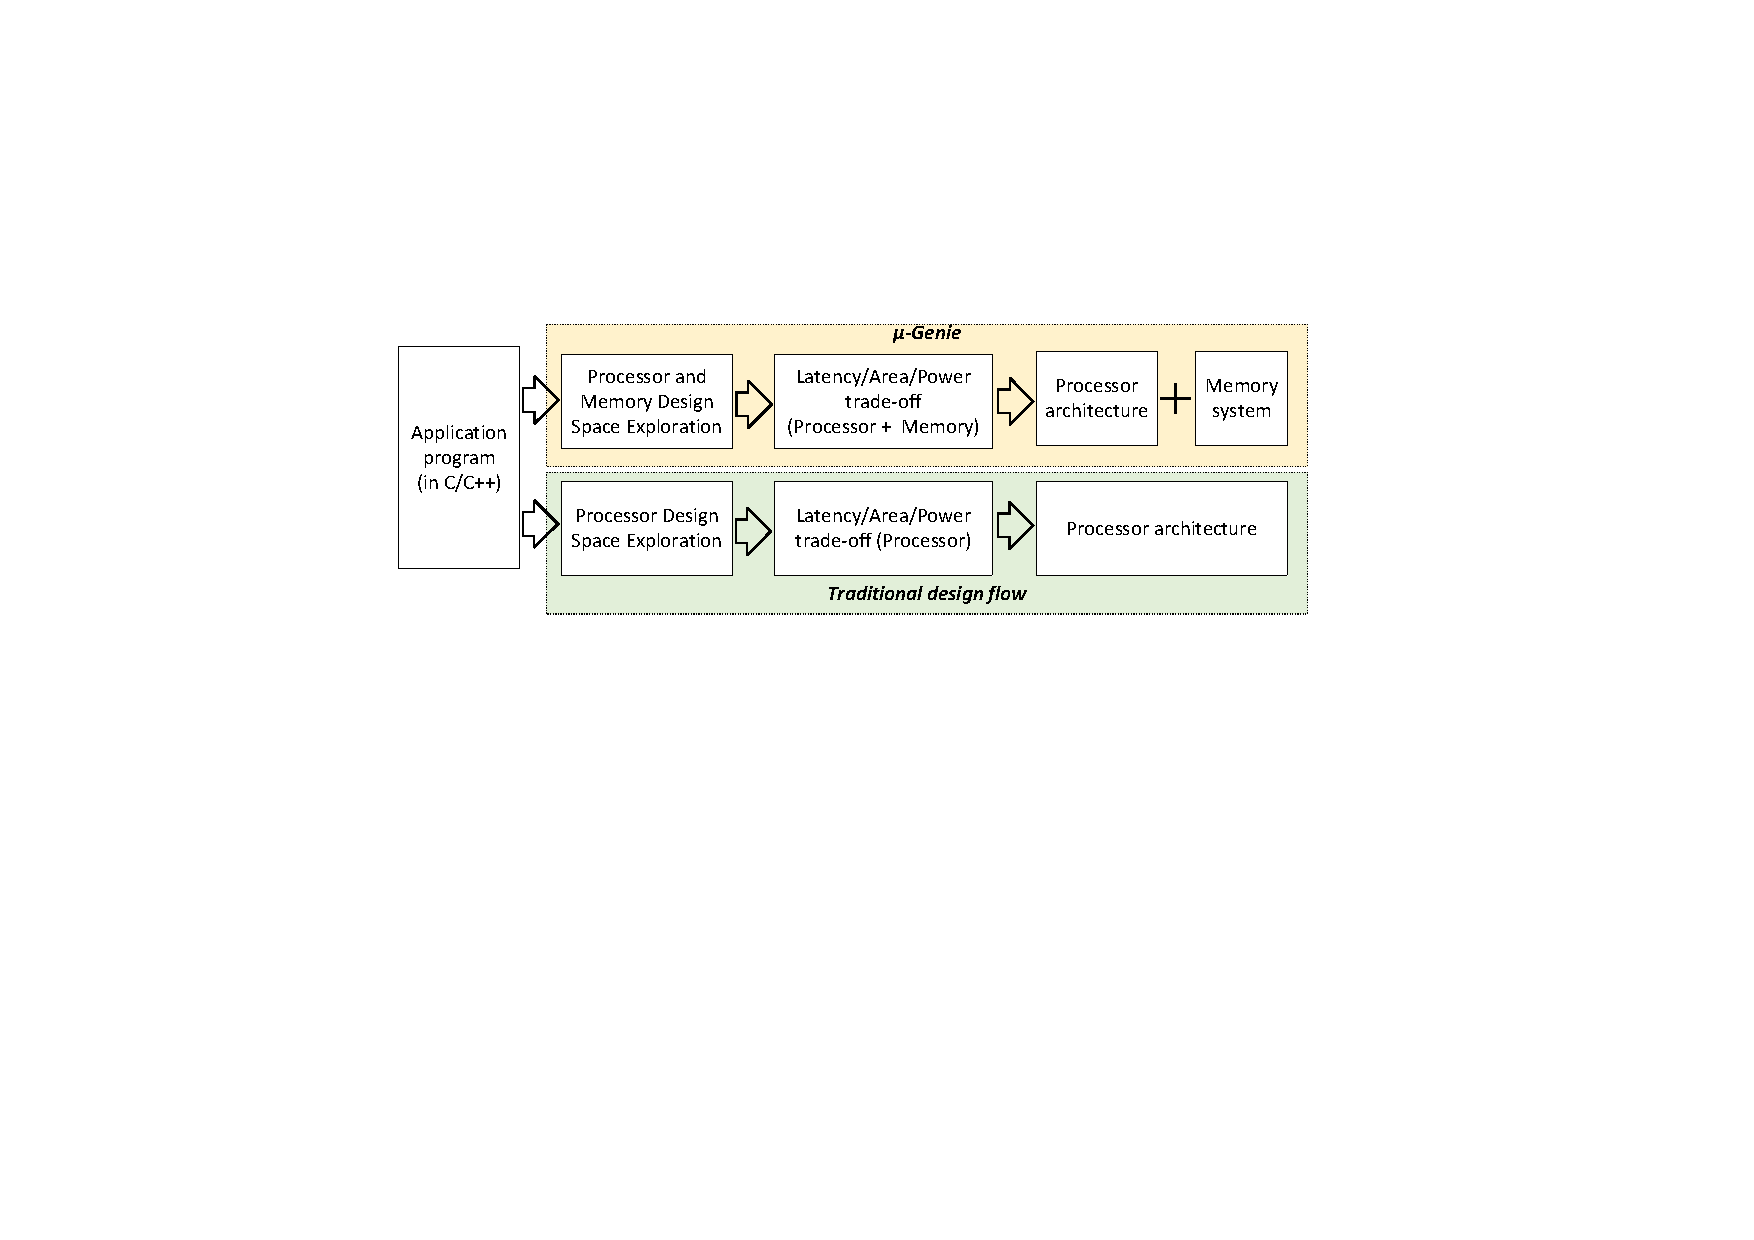
\includegraphics[clip, trim=6cm 10.5cm 6.4cm 5.2cm, width=1.0\linewidth]{images/intro_figure.pdf} %[left down right up ] 
    \caption{\small Difference between state-of-the-art and the proposed \frameworkname~design flows for custom processor architecture design.}
    \label{fig:intro}
\end{figure}

In this work, we propose \frameworkname (\ref{sec:framework}), a novel automated framework for \textit{memory-aware custom-processor design-space exploration}, which enables users to explore various architectural trade-offs for the joined (processor, memory system) ensemble. The framework allows unprecedented configuration options: memory levels technologies (novel among similar tools), clock frequency (per memory level, also novel), read/write latency (potentially different), and data width. Thus, our \frameworkname~is the first to enable design-space exploration for application-specific custom-processors beyond state-of-the-art solutions, even enabling a first comparison between different memory technologies, like MRAM and SRAM (Section~\ref{sec:case_studies}).

Moreover, \frameworkname~uses spatial architectural templates (Section~\ref{sec:arch_template}) to actually generate ready-to-use custom-processor designs. These designs can be configured at design-time (based on the trade-off from the framework), and allow for fast prototyping of application-specific hardware.  

To demonstrate the capabilities of \frameworkname, we covers three case-studies, showing how custom-processor designs for two different applications and many configurations, even those using MRAM or SRAM for the memory system, can be generated, analysed, and compared (Section~\ref{sec:case_studies}).
 
 %Ana: if you keep this format, without the contributions specifically listed, this final paragraph (below) is not well-positioned. You might want ti add this at the beginning of "In this work..." paragraph - I added it there for you to see what I mean. This summary is only needed here if you go for the bullet-point-like contributions.  
 %\frameworkname~enables design space exploration for application-specific custom-processors beyond the current state-of-the-art solutions, even enabling a first comparison between different memory technologies, like MRAM and SRAM.

%In this work we present \frameworkname, a framework that allows to compare design choices and perform automatic system level design and implementation. We propose a novel memory-driven approach for application-specific hardware design starting from two observations. First, the memory system and the processing system are \textit{interdependent} and therefore they should be \textit{co-designed}. Second, the \textit{data dependencies} of the fixed application impose constaints on the design of both memory and processing systems. Hence, our approach starts from the analysis of an input application and codesigns memory and custom processor, shown in Figure~\ref{fig:intro}. 





%TODO, remove figure or reuse the one in [1] and update accordingly the terminology
\section{Background}
\label{sec:bg}

A \textit{spatial processor} architecture consists of a set of physically distributed PEs with dedicated control units interconnected using an on-chip interconnect. The operations that need to be performed by an algorithm are mapped on the PEs, which compute in a fine-grained pipeline fashion. There are different kinds of spatial architectures, one possible classification is shown in Figure \ref{fig:spatial_class}\cite{parashar2014efficient}. FPGAs are an example of spatially programmed architecture in which the PEs implement basic logic operations, and hence are classified as Logic-Grained. To change the functionality of a Logic-Grained architecture, the hardware design needs to be modified and re-synthesized. Instruction-Grained spatial architecture are instead programmable at instruction level and their PEs implement simplified ALUs. The functionality of a \textit{Instruction-Grained} spatial accelerator can change by modifying the sequence of instructions it executes. The advantage of using \textit{Instruction-Grained} over \textit{Logic-Grained} programmable architectures lies in their higher computational density, which results in a higher operational frequency and lower power consumption\cite{parashar2014efficient}. The Instruction-Grained class is itself composed of architecture having Centralized Control\cite{swanson2007wavescalar} , where a single control unit manages all the PEs, and Distributed Control, where each PE has a built-in control mechanism~\cite{parashar2014efficient,prabhakar2017plasticine,cerqueira2020catena}. Intuitively, an architecture with distributed control is more scalable and has a simpler interconnection network.
In this work we introduce \frameworkname, an automated framework that \textit{generates distributed control spatial architectures optimized for input applications}.




\begin{figure}
  \centering
  \resizebox{0.5\columnwidth}{!}{%
    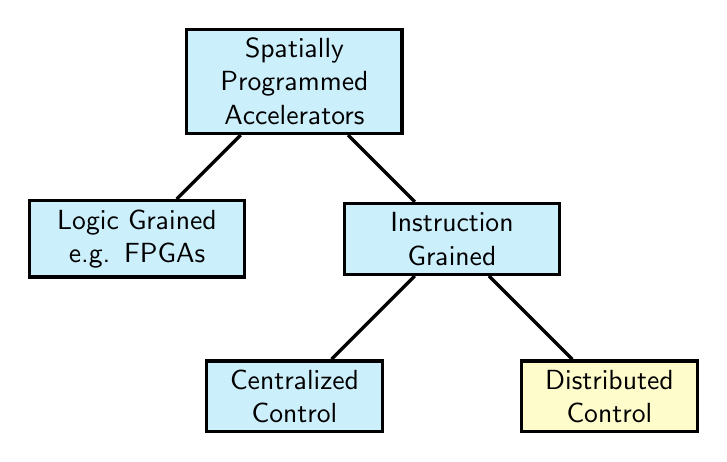
\begin{tikzpicture}[
      % For compatability with PGF CVS add the absolute option:
      absolute
      ]
      \begin{scope}[xshift=-7.5cm,yshift=-5cm,very thick,
        node distance=2cm,on grid,>=stealth',
        block/.style={rectangle,draw,font=\sffamily,fill=cyan!20,text width=2cm,text centered}]

        \node[block, text width=2.5cm] (spatial_acc) {Spatially Programmed Accelerators};
        \node[below=of spatial_acc]  (dummy1){};
        \node[block, left=of dummy1,text width=2.5cm] (logic_grain) {Logic Grained\\e.g. FPGAs};
        % \node[below=of logic_grain,yshift=35pt] (fpga) {FPGAs};
        \node[block, right=of dummy1, text width=2.5cm] (inst) {Instruction Grained};
        \node[below=of inst] (dummy2){};
        \node[block, left=of dummy2] (cent_ctrl) {Centralized Control};
        \node[block, right=of dummy2,fill=yellow!20] (dist_ctrl) {Distributed Control};
        \draw[-] (spatial_acc) -- (logic_grain);
        \draw[-] (spatial_acc) -- (inst);
        \draw[-] (inst) -- (cent_ctrl);
        \draw[-] (inst) -- (dist_ctrl);
      \end{scope}

    \end{tikzpicture}
  }
  \caption{Spatial Architectures classification \cite{parashar2014efficient}.} \label{fig:spatial_class}
\end{figure}

%This section will contain the relevant background. Consider the following items:
%\begin{itemize}
%\item Taxonomy of accelerators
%\item Non-Volatile Memories
%\item Memory wall
%\item Static Data-Dependency Analysis
%\item System Under Analysis
%\end{itemize}

\begin{figure*}[!ht]
\begin{minipage}{.7\textwidth}
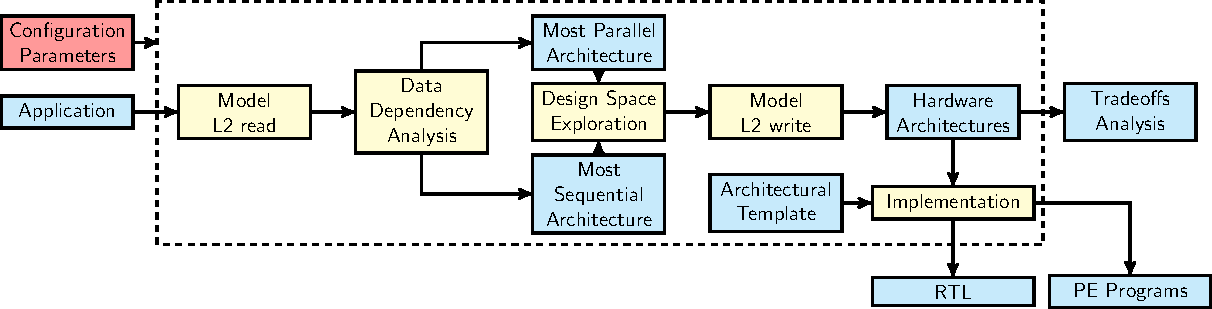
\includegraphics[width=\textwidth,left]{images/framework_v2.pdf}
  \caption{\small \frameworkname~Framework.}{}
  \label{fig:framework}
\end{minipage}%
\begin{minipage}{.3\textwidth}
    \centering
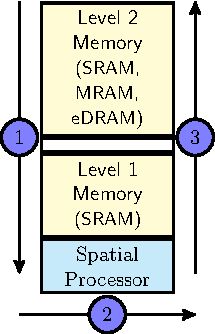
\includegraphics[width=.4\textwidth]{images/architecture_v2.pdf}
\caption{\small The system under analysis.
    }
\label{fig:system}
\end{minipage}
\squeezeup
\squeezeup
\end{figure*}
\section{The \frameworkname~framework}
\label{sec:framework}
The \frameworkname~framework, illustrated in Figure~\ref{fig:framework} takes two inputs, the \textit{Configuration Parameters} and an \textit{Application} - described in Section~\ref{ssec:app}, and automatically generates a set of hardware architectures, behaviorally equivalent to the input application.
%Ana: the sentence below was a repetition - can skip.
%Additionally, the analysis of area, power and latency of these architectures is automatically produced.
The generated hardware architectures can be realized as RTL implementations, using the \textit{architectural templates} described in Section~\ref{sec:arch_template}.
The rest of this section provides an overview of the design and implementation of \frameworkname.

%\vspace{-1mm}
%\subsection{Model of Execution}
\label{ssec:system_under_analysis}
%\vspace{-1mm}
The system architecture we assume in this work has two levels of memory and a spatial processor (Figure~\ref{fig:system}). Level 1 memory (L1M)\footnotemark, the first memory level, and the smaller one in size, uses SRAM as it needs to be physically close to the processor for faster access. The second level - Level 2 memory (L2M)\footnotemark[\value{footnote}] - is larger in size and can be implemented using any memory technology (on-chip or off-chip), even with different access latency for read and write operations. Note that L2M can run at a different clock speed and different IO width than the processor and L1M.
\footnotetext{These memories are not to be seen as caches; thus, no cache policies are needed: we schedule data movements at design time. This is why we call them "levels" instead of "layers", and we abbreviate them with L1M and L2M instead of L1 and L2.}


We assume a model of execution following the three steps from Figure~\ref{fig:system}. Initially, all the required input data for the application are available in L2M. The input data is transferred to the processor, using L1M as intermediate storage (step 1), the data is processed and the results are temporarily stored in L1M (step 2), and, finally, the data from L1M is transferred back to L2M (step 3). The data transfers between L2M and L1M are handled by a Direct Memory Access (DMA) controller. Note that our model of execution performs the steps in a pipelined manner, hence only part of the data will be stored in L1M at any given time.

%\frameworkname~lets the user specify the parameters of the L2M through the \textit{Configuration Parameters}. The L2M parameters are used to model the data transfer between L2M and L1M (see \ref{ssec:layer2_model} and \ref{ssec:l2_read_model}). The L2M model is used to compute arrival time of input elements in the L1M. The arrival time of the element in the L1M is then used by the Modified Interval Partitioning (MIP) algorithm  - see \ref{ssec:modified_interval_partitioning}, to produce spatial architectures having bandwidth close to the bandwidth of the L2M. This effectively reduces the instantiation of unrequired resources in both the L1M and the spatial processor.
%The L1M is composed of multiple banks having different depths. The number and depths of the banks composing the L1M is determined by the MIP as described in \ref{ssec:arch_tradeoffs}.

%Taking advantage of the possibility to produce stacked chip having levels produced using different manufacturing technologies we are able to explore different memory implementations at the L2 of the memory architecture.

%\begin{figure}[tb]
%\centering
%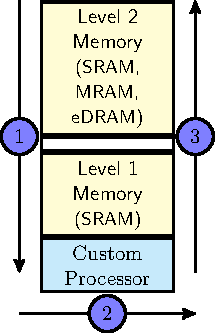
\includegraphics[width=0.25\columnwidth]{images/architecture.pdf}
%\caption{\small The system under analysis. Composed by two levels of memory, the memory at layer two can use various technologies while the memory at layer one uses only SRAM technology.}
%\label{fig:system}
%\end{figure}

%\vspace{-1mm}
%\subsection{The L2 Memory Model}
\label{ssec:layer2_model}
%\vspace{-1mm}
Because L2M has higher access latency compared to the L1M and spatial processor, we model the L2M assuming its data is accessed in bursts.
%Figure~\ref{fig:l2model}  shows a representation of such access.
A read or write burst access to the L2M is controlled by a Direct Memory Access (DMA) controller, with the starting address and size of the burst given as input to the DMA. After an initial \textit{setup latency}, the accessed elements are transferred in sequence from the start address to the end address, from L1M to L2M in case of a write, and from L2M to L1M in case of a read.

\section{\frameworkname: Inputs}
This section details the two inputs of \frameworkname: the \textit{application} and the \textit{Configuration Parameters}.
%\vspace{-1mm}
%\subsection{Application}
\label{ssec:app}
%\vspace{-1mm}
The applications that can be used as input to \frameworkname~are completely defined at compile time, having control-flow instructions not dependent on input data. Such applications allow the static extraction of data dependency information performed by the \textit{Data Dependency Analysis} module (\ref{ssec:dda}). We currently support C/C++ applications. However, as the framework uses the LLVM Intermediate Representation~\cite{llvm}, it can be easily extended to support other languages as well.
%\begin{lstlisting}[language=C, caption={Example of input application, C implementation of a matrix vector multiplication.}, label={lst:matrixvec}]
%void matrix_vec_kernel(int *A,int *B, int *C){
%    int sum;
%    for(int i=0;i<DIM2;i++){
%        sum=0;
%        for(int j=0;j<DIM1;j++){
%            sum+=A[i*DIM1+j]*B[j];
%        }
%        C[i]=sum;
%    }
%}
%\end{lstlisting}

%\vspace{-1mm}
%\subsection{Configuration Parameters}
\label{ssec:conf_param}
%\vspace{-1mm}
The second input to the framework is a configuration file for the different building blocks to be used for hardware architecture realization. Through this file, the user can specify: different compute units (e.g. multipliers, adders), process technology to be used (e.g. 16nm, 28nm), the clock frequency of the processor and L1M, and the clock frequency L2M. Moreover, the user can specify the data-width used by the compute units, L1M and L2M.
Information to model the L2M burst accesses is also specified in this file: the setup latency for write/read accesses, the type of L2M to be used (e.g. MRAM, SRAM) and the size of the L2M. The different parameters in the configuration file are then used to access a database containing estimates (obtained by synthesis or from specs) of area usage, static and dynamic power, and latency of each of the building blocks. %Our L1M implementation uses multiple memory banks of different sizes (see \ref{ssec:arch_tradeoffs}). To estimate the resource usage of the different types of these memories we built a linear model, using synthesis data. We compared the ability of our linear model to predict area, latency and power consumption against the data generated using the synthesis tool and we found it to be accurate - less then 2\% error in the area and static energy model and less than 28\% error in the dynamic energy model.

%\begin{lstlisting}[language=json, caption={Example of input configuration file}, label={lst:conf_file}]
%{
%   "resource_database": {
%	"technology": 16,
%	"clock_frequency": 1000,
%	"bitwidth_adder": 128,
%	"bitwidth_multiplier": 64,
%	"bitwidth_register_file": 128,
%	"type_l2": "tt1v1v85c",
%	"technology_l2": 16,
%	"clock_l2": 800,
%	"bitwidth_l2": 32,
%	"depth_l2":2048,
%	"setup_write_latency_l2":2,
%	"setup_read_latency_l2":2
%   }
%}
%
%\end{lstlisting}

\section{\frameworkname: Analysis}
This section describes the parts of the framework involved in modeling the data transfers between L2M and L1M, \textit{Model L2 read} and \textit{Model L2 write} (\ref{ssec:l2_read_model}), the modules that perform data dependence analysis, \textit{Data Dependency Analysis} (\ref{ssec:dda}), and the scheduling of the application operations (\ref{ssec:modified_interval_partitioning}).
\vspace{-1mm}
\subsection{L2 Memory Read and Write Modeling}
\label{ssec:l2_read_model}
\vspace{-1mm}
The first operation performed by the framework is to compute the transfer time of the application's input data from L2M to L1M, implemented in the \textit{Model L2 read} block of Figure \ref{fig:framework}. Using static analysis, we obtain details regarding the data structures used in the application. For example, in a matrix vector multiplication kernel, the static analysis extracts information about three data structures: an input matrix and an input vector, containing the input elements of the computation, and an output vector containing the results. An address in L2M is given to each input element used by the application; different data structures are placed in consecutive memory addresses. The entire data transfer is modeled as a single burst-read operation from L2M. The information required to compute the arrival clock cycle of each input element to L1M is extracted from the \textit{Configuration Parameters}.
Using this information, the exact clock at which each input element arrives in L1M can be computed as seen in (1). The equation symbols are described in Table~\ref{table:equation}.

\begin{equation}
AClk_i = S_r + R_{L2M} * (Add_{L2Mi}+1) * \frac{B_{L1M}}{B_{L2M}} * \frac{Clk_{L1M}}{Clk_{L2M}}
\end{equation}

\begin{table}[]
\centering
%\footnotesize
\scriptsize
\begin{tabular}{|l|l|}
\hline
\textbf{Symbol} & \textbf{Definition}                                           \\ \hline
$AClk_i$           & Clock at which element i arrives to L1M                \\
$S_r$             & Setup Latency of a L2M burst read                          \\
$R_{L2M}$       & L2M read latency (per read), in L2M clock cycles   \\
$Add_{L2Mi}$     & Offset of element i in the burst access \\
$B_{L1M}$        & Data bitwidth of L1M                                       \\
$B_{L2M}$        & Data bitwidth of L2M                                       \\
$Clk_{L1M}$      & Clock Frequency of L1M                                     \\
$Clk_{L2M}$      & Clock Frequency of L2M                                     \\
$WBL_{L2M}$      & L2M write burst latency                                    \\
$S_w$             & Setup Latency of a L2M burst write                         \\
$W_{L2M}$       & L2M write latency (per write) in L2M clock cycles  \\
$O$                 & Total number of output elements                            \\ \hline
\end{tabular}
\caption{\small Definition of symbols used in the equations}
\label{table:equation}
\squeezeup
\squeezeup
\end{table}
The schedule produced by the Modified Interval Partitioning (MIP), discussed in \ref{ssec:modified_interval_partitioning}, uses the arrival clock cycle computed in this phase to determine when each input element will be available for computation in L1M. The latency of the MIP schedule includes therefore the L2M$\rightarrow$L1M transfer, and the computation; it does not take into account the L1M$\rightarrow$L2M transfer of the results (phase 3 in Figure~\ref{fig:system}).
The \textit{Model L2 write} block in Figure \ref{fig:framework} computes the latency of the L1M$\rightarrow$L2M transfer. The MIP computes the clock cycle at which computation ends (phase 2 in Figure~\ref{fig:system}) and the last data item is written in L1M. The L1M$\rightarrow$L2M transfer can start immediately after the last output is generated.
The latency of the L1M$\rightarrow$L2M transfer is calculated using (2),
\begin{equation}
    WBL_{L2M} = S_w + W_{L2M} * O * \frac{B_{L2M}}{B_{L1M}} * \frac{Clk_{L1M}}{Clk_{L2M}}
\end{equation}
where the symbols have been defined in Table~\ref{table:equation}.


\vspace{-1mm}
\subsection{Data Dependency Analysis}
\label{ssec:dda}
\vspace{-1mm}
The \textit{Data Dependency Analysis (DDA)} module operates in three stages. The first two stages are the extraction of the \textit{Data Dependency Graph} (DDG)\cite{isoda1983global} from the application and the schedule of the DDG using the As Soon As Possible (ASAP) and As Late As Possible (ALAP) methodologies. These two steps are core elements in the analysis of high level code for hardware design\cite{hwang1991formal}. Finally, the third step (see \ref{ssec:modified_interval_partitioning}) maps DDG instructions to hardware components - or PEs - using a modified \textit{Interval Partitioning} algorithm~\cite{greedyIntervalPartitioning}.
%This next paragraph might be replaced with a reference

%To extract the DDG from an application, we use LLVM  and custom transformations. We first convert the input application code to its LLVM Intermediate Representation. We then transform the code into static single assignment (SSA) form and perform full-loop unrolling on all of the application loops. After these transformations, there will be no control flow instructions in the application body, and each variable will be defined only once. It is now possible to follow the definition and use chain of the variables to produce a Data Dependency Graph like the one shown in Figure~\ref{fig:ddg}. The DDG represents each operation as a node - in Figure~\ref{fig:ddg} the input and output nodes represent respectively load and store instructions, while oval nodes represent computations - and each edge represents a dependency between operations.

We extract the DGG from the application using some LLVM optimizations and some custom code. We further process the obtained DDG, aiming to reduce the length of the path between the input nodes and the output nodes. This additional transformation is important because the length of these paths is equivalent to the number of sequential operations required to obtain the outputs, which in turn determines the latency of the application. Taking advantage of operation associativity (where possible) we can transform a long sequence of operations - like the one highlighted in Figure~\ref{fig:ddg} - into an equivalent shorter tree.
%\begin{figure}[ht]
%\begin{minipage}{.5\textwidth}
%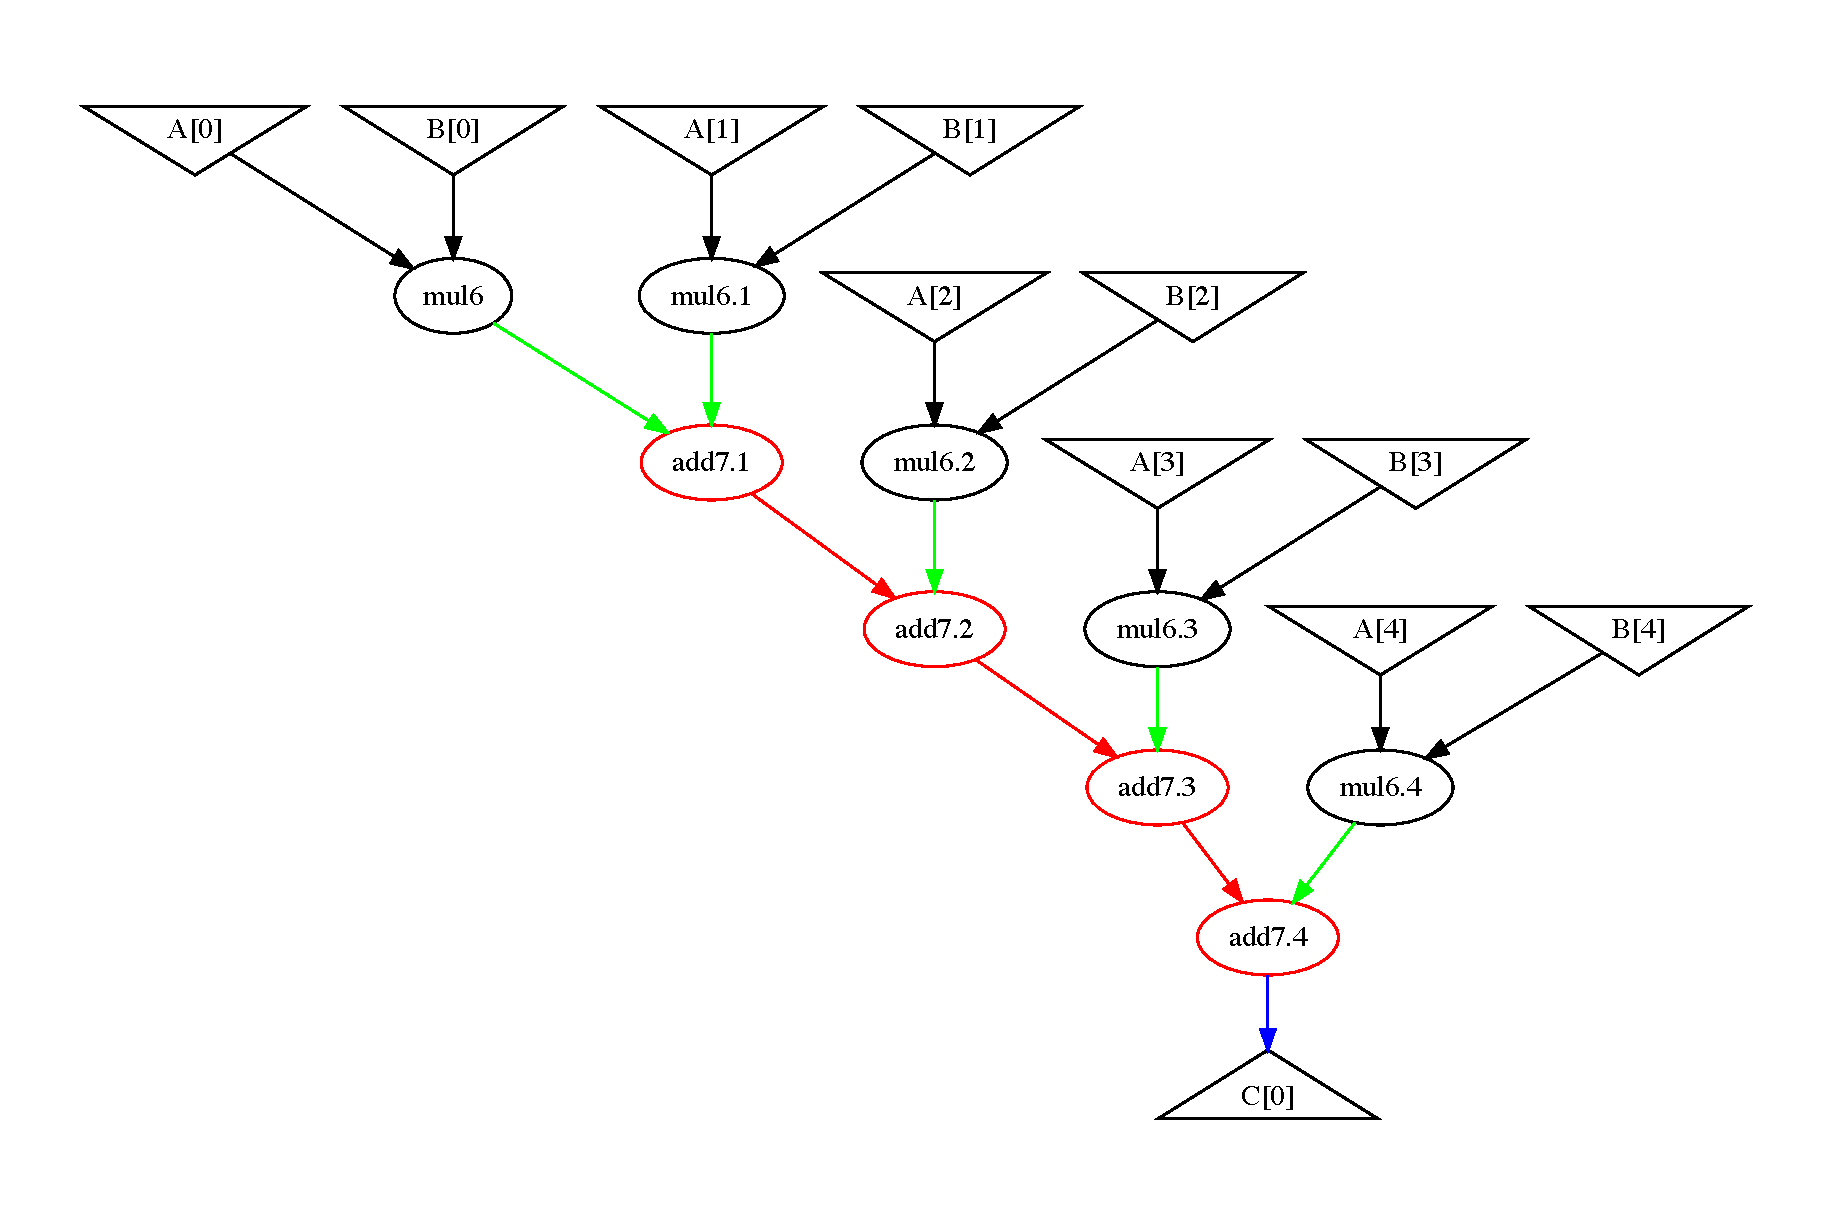
\includegraphics[width=.9\textwidth,left]{images/supernode.pdf}
%  \caption{\small \frameworkname~Framework.}{}
%  \label{fig:framework}
%\end{minipage}%
%\begin{minipage}{.5\textwidth}
%    \centering
%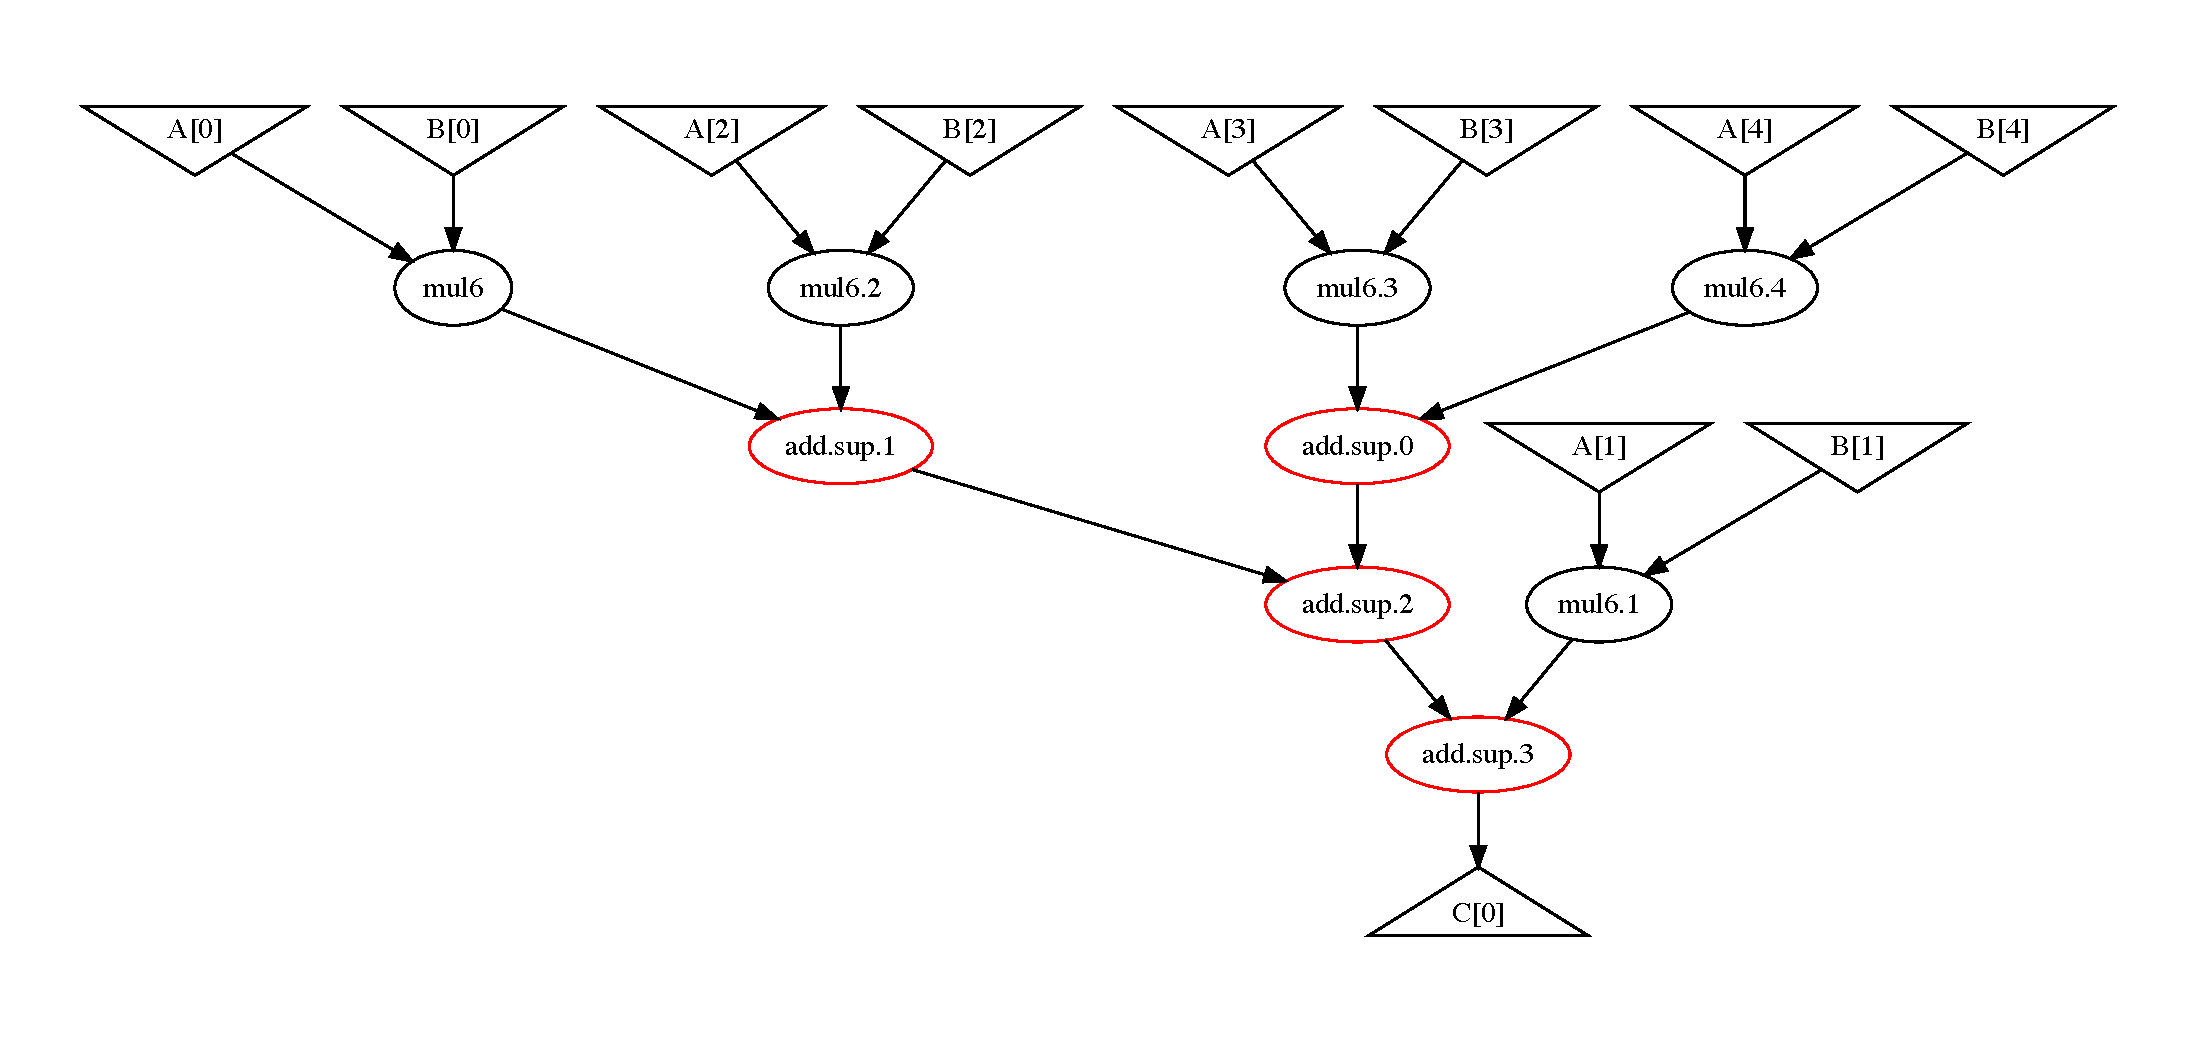
\includegraphics[width=.9\textwidth]{images/supernode_optimized.pdf}
%\caption{\small The system under analysis.
%    %Composed by two levels of memory, the memory at layer two can use various technologies while the memory at layer one uses only SRAM technology.
%    }
%\label{fig:system}
%\end{minipage}
%\end{figure}

\begin{figure}[tb]
\centering
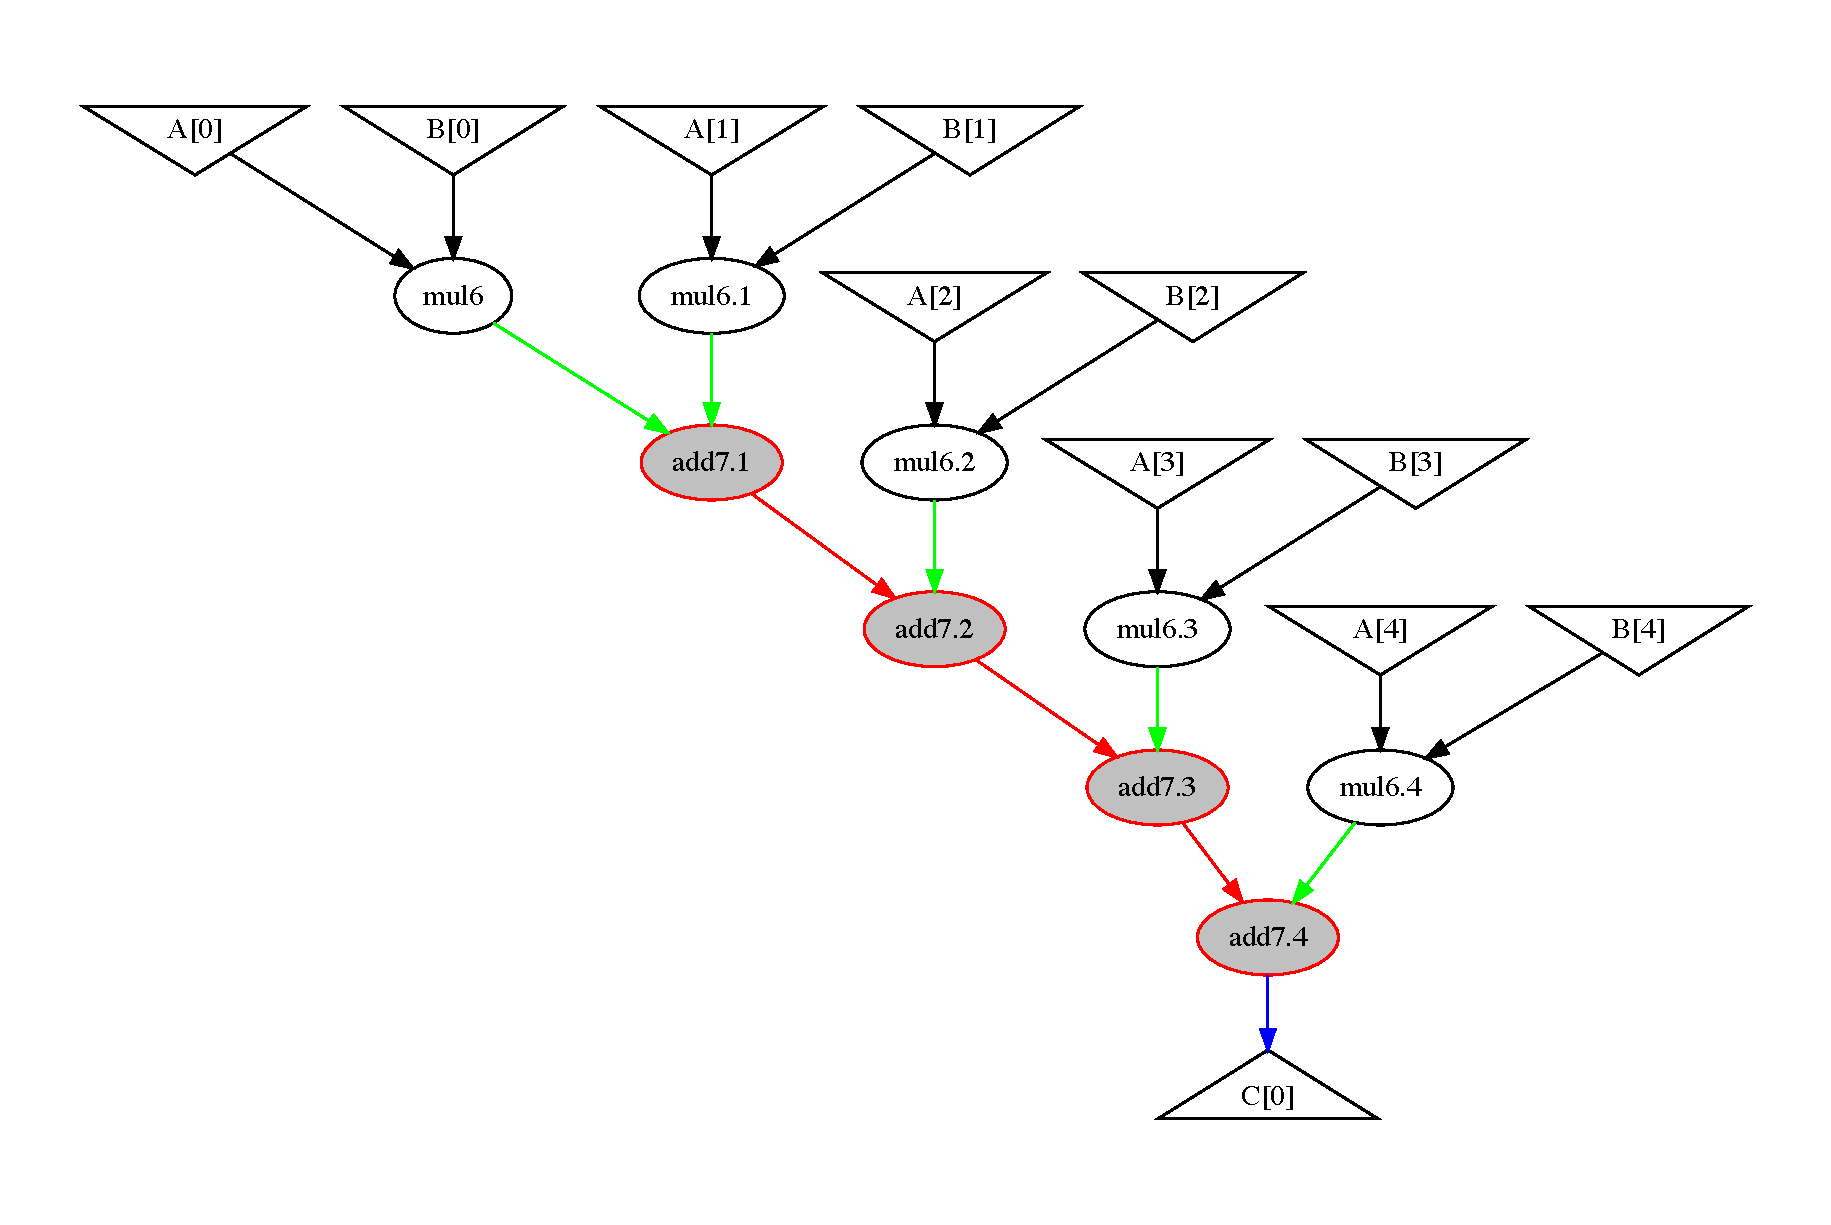
\includegraphics[width=.9\columnwidth,left]{images/supernode_2.pdf}
\caption{\small A Data Dependency Graph: inverse triangles represent input data, obtained from the \textit{load} instructions; ovals describe operations on data; the triangle at the bottom represents the result, derived from a \textit{store} instruction. Highlighted, a chain of associative operations before being optimized by the \textit{DDA} module (\ref{ssec:dda}).}
\label{fig:ddg}
\end{figure}

%This next paragraph might be replaced with a reference, we are interested mainly in the concept of mobility
Next, we apply the ASAP and ALAP scheduling methodologies\cite{hwang1991formal} to the generated DDG. These schedules will associate to each DDG node a clock cycle where the instruction is executed, and \textit{bound} the design space of possible architectures by determining the \textit{maximally parallel} architectures. We start by scheduling the input nodes of the DDG using the arrival clock time of their input data, computed as explained in Section~\ref{ssec:l2_read_model}, thus taking into account the L2M - L1M transfer time. Next, we determine the minimal latency required to obtain the outputs of the application with the ASAP schedule: starting from the DDG input leafs, each instruction node is scheduled as soon as its dependencies are resolved.
Once ASAP is completed, we can perform the ALAP scheduling: starting from the output leaf nodes, each node is scheduled as late as possible according to its dependencies. Once ALAP is completed, every node is annotated with an ASAP clock cycle and an ALAP one. The difference between these two clock cycles, called instruction \textit{mobility}, identifies an interval in which the instruction can be scheduled without changing the overall latency of the application.

The final stage of the \textit{Data Dependency Analysis} module will allocate the DDG nodes to PEs, leveraging the nodes mobility to minimize the number of PEs of the final hardware architecture.

\vspace{-2mm}
\subsection{PE allocation with Modified Interval Partitioning}
\label{ssec:modified_interval_partitioning}
\vspace{-1mm}
To generate a hardware architecture behaviorally equivalent to the input application and with the latency identified during the ASAP-ALAP scheduling, there are two main requirements: (1) each instruction needs to be computed within its ASAP-ALAP interval, and (2) instructions in the DDG which are executed by the same PE cannot be scheduled at the same time.
Our Modified Interval Partitioning (MIP) algorithm - based on the original greedy Interval Partitioning algorithm~\cite{greedyIntervalPartitioning} - is designed to generate, from a DDG, hardware architectures that meet both requirements. The original Interval Partitioning problem addresses the issue of assigning a number of jobs, with known starting and ending time, to the minimum amount of resources, ensuring that the jobs assigned to a resource do not overlap.


To use Interval Partitioning for our problem, we consider instructions as jobs and PEs as resources. There are, however, three main differences between our problem and the canonical Interval Partitioning.
First, the original algorithm considers any job can use any resource, while our architecture requires different PEs for different instructions. We therefore perform interval partitioning several times, once for each instruction type (e.g., four times for the graph in Figure \ref{fig:ddg}). This ensures a correct allocation of instructions to PEs performing the same operation.
Second, due to \textit{mobility}, instructions do not have a fixed starting time. MIP takes the mobility of an instruction into account by allowing a given instruction to start at any time within its allowed interval.
Third, our instructions are dependent on each other, which is not the case for the jobs in the original interval partitioning. To account for this extra constraint, we ensure that any given instruction (a) is only allocated after its dependencies are allocated, and (b) is scheduled to start after the ending time of its dependencies.
%Listing~\ref{lst:modified_interval_partitioning} presents MIP, in pseudo-code. %of our modified interval partitioning algorithm.

%\begin{lstlisting}[language=Python, caption={\small Modified Interval Partitioning (MIP) Algorithm}, label={lst:modified_interval_partitioning}, basicstyle=\tiny]
%# ASAP[i] and ALAP[i] contain the scheduled cycles for instruction i
%# SetPEs is the set of Processing Elements in the architecture
%SetPEs=[]
%sort instructions by ASAP[i]
%for each instruction i%
%	allocated = False
%	dep_deadline = maximum end-time of all instructions depending on i
%	schedule[i] = max(ASAP[i], dep_deadline)
%	for each PE in SetPEs
%		if instruction i matches PE
%			if ALAP[i] >=  next_free_slot[PE]
%				add instruction i to PE
%				schedule[i] = max(schedule[i], next_free_slot[PE])
%				next_free_slot[PE] = schedule[i] + latency(i)
%				allocated = True
%	if not allocated
%		create new PE with type(i)
%		add instruction i to PE
%		next_free_slot[PE] = schedule[i] + latency(i)
%		add PE to setPEs
%\end{lstlisting}

%We assume that ASAP and ALAP schedules have been previously performed, hence we can have two data structures that return the ASAP and ALAP schedules for a given instruction i - i.e. ASAP[i] and ALAP[i].
%Instructions is an ordered list of instructions initialized with the instructions of the input application.
%A Functional Unit is represented as a set containing the instructions that have been allocated to it, and FunctionalUnits is a set containing the Functional Units of the resulting architecture which is initialized as an empty set.
%The functions latency and dep take an instruction i as input and return respectively the latency of i and a list of instructions i depends on.
%The function type takes as input a Functional Unit or an Instruction and returns the type of operation performed.

%The MIP algorithm returns \verb|setPEs| and a \verb|schedule| for the current design: \verb|setPEs| is the list of processing elements that form the architecture, with each PE containing the instructions it has to execute, while \verb|schedule| contains the clock cycle at which each instruction is scheduled to be executed.

\vspace{-1mm}
\subsection{Most Parallel and Most Sequential Architectures}
\vspace{-1mm}
The result of the \textit{DDA} module is the \textbf{Most Parallel Architecture (MostPar)}. This architecture takes full advantage of the parallelism of the application and performs the computation with the minimum latency. However, MostPar uses the maximum number of PEs - in the worst case scenario equivalent to the number of instructions in the application - and it will hence have the largest area.
At the other end of the spectrum of architectures we can imagine the \textbf{Most Sequential Architecture (MostSeq)}, where no parallelism is used and the instruction are scheduled sequentially respecting their dependencies. This architecture will have the worst possible latency, but the minimal impact in area - using only one PE per operation type.
Probably none of these two architectures will be of direct interest for the user as they represent two extreme cases. Instead, the interesting architectures are the ones \textit{in between} \textbf{MostSeq} and \textbf{MostPar}, because they offer interesting trade-offs between power, latency and area. Section~\ref{ssec:dse} describes how these intermediate architectures can be generated using \textbf{MostPar} and \textbf{MostSeq}, respectively, as upper and lower bounds of the design space.

\section{\frameworkname: Design Space Exploration (DSE)}
%\vspace{-1mm}
%\subsection{Design Space Exploration}
\label{ssec:dse}
%\vspace{-1mm}
The \textit{Design Space Exploration} \frameworkname~module generates hardware architectures, behaviorally equivalent to the input application, which exhibit area, latency and power tradeoffs.
Our DSE is an iterative process which produces, at the end of each iteration, a different hardware architecture.
The iterative process starts its sweep from \textbf{MostPar}, and ends when \textbf{MostSeq} is generated.
%\begin{lstlisting}[language=Python, caption={\small Design Space Exploration},label={lst:dse},basicstyle=\tiny]
%currentArchitecture = MostPar
%found_MostSeq=False
%GeneratedArchitectures=[]
%while(!found_MostSeq)
%    type_count={}
%    found_MostSeq=True
%    for each PE in currentArchitecture
%        type_count[type(PE)]+=1
%            if type_count[type(PE)] > 1
%                found_MostSeq=False
%                break
%    if found_MostSeq
%       break
%    for each instuction i in DDG
%        if type(i) == 'store'
%            ALAP[i] = ALAP[i]+1
%    ALAP=performALAPschedule(instructions,dependencies)
%    SetPEs=MIP(instructions,ASAP,ALAP)
%    GeneratedArchitectures+=[SetPEs]
%    currentArchitecture=SetPEs
%\end{lstlisting}
An iteration consists of three steps. First, the instructions corresponding to output leaf nodes in the DDG are selected. The ALAP schedule of these iterations is increased by 1, and the ALAP scheduling of the rest of the nodes in the DDG is updated accordingly. Consequently, the mobility of each instruction node is increased by one. Finally, the MIP is ran again, using the new ALAP schedule. Due to the increased mobility of each instruction, the generated architecture is likely to use less PEs.
The process stops as soon as it generates \textbf{MostSeq}, which can be recognized because it contains only one PE per operation type.

Users can tune the DSE process, trading speed for completeness: by increasing the ALAP "slack" beyond 1, the exploration speeds-up, but less architectures are generated.

%This has been merged with the L2 Memory Read section
%\vspace{-1mm}
%\subsection{L2 Memory Write}
%\vspace{-1mm}
%The schedule produced by MIP includes the L2M-L1M transfer, and the computation; it does not include the L1M-L2M transfer. However, due to MIP, we do know the clock cycle at which computation ends (phase 2 in Figure~\ref{fig:system}) and the last data item is written in L1M. The L1M-L2M transfer can start immediately after the last output is generated.
%The latency of the L1M-L2M transfer is calculated using (2),
%\begin{equation}
%    WBL_{L2M} = S_w + W_{L2M} * O * \frac{B_{L2M}}{B_{L1M}} * \frac{Clk_{L1M}}{Clk_{L2M}}
%\end{equation}
%where the symbols have been defined in Table~\ref{table:equation}


%\vspace{-1mm}
%\subsection{Architecture Tradeoffs}
%\label{ssec:arch_tradeoffs}
%\vspace{-1mm}
%In section~\ref{
%For a given input application and a given configuration, \frameworkname~outputs a set of hardware architectures - composed of spatial processor and L1M - with different area and latency trade-offs. Figure~\ref{fig:tradeoffs} shows three of the architectures generated during the DSE. Each box represents a PE. The different load and store PEs are implemented as separate L1M banks. As an example, the architecture in Figure \ref{fig:inter_arch} has 1 L1M bank to store the input data and 5 banks to store the results. This architecture can therefore receive 1 input element per clock cycle from the L2M, and store up to 5 results per clock in the L1M store banks. The remaining PEs are obtained from computing instructions. We allow the architectures to have cycles because the circuit is synchronous, and every instruction has been carefully scheduled. A self-loop in a PE indicates data reuse (see Section~\ref{sec:arch_template} for implementation details).
%\begin{figure}[ht]
%\centering
%\begin{subfigure}{.4\columnwidth}
%  \centering
%  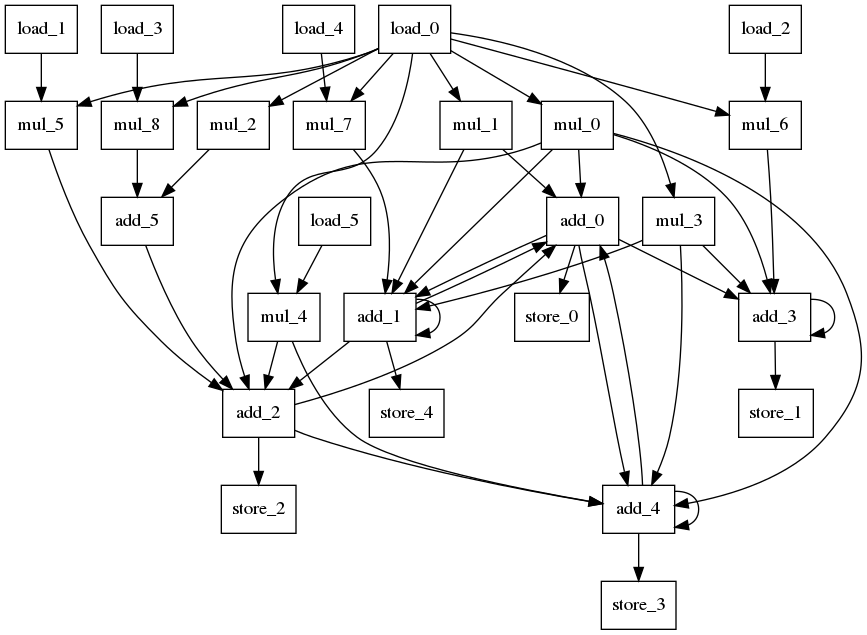
\includegraphics[width=\textwidth]{images/Architecture_latency_146_schematic.png}
%  \caption{}
%  \label{fig:max_par_arch}
%\end{subfigure}%
%\begin{subfigure}{.3\columnwidth}
%  \centering
%  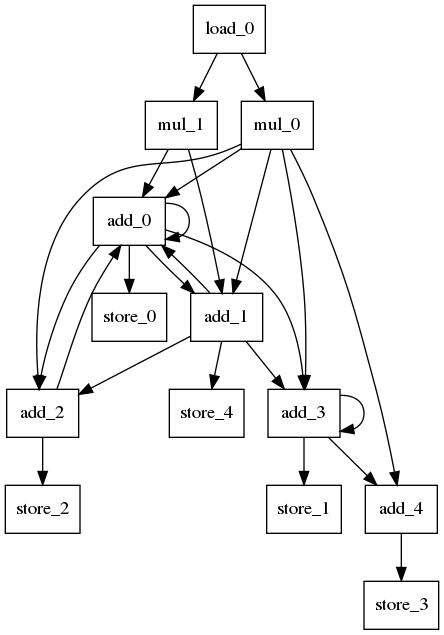
\includegraphics[width=\textwidth]{images/Architecture_latency_166_schematic.png}
%  \caption{}
%  \label{fig:inter_arch}
%\end{subfigure}
%\begin{subfigure}{.2\columnwidth}
%  \centering
%  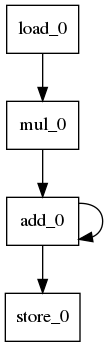
\includegraphics[width=0.5\textwidth]{images/Architecture_latency_188_schematic.png}
%  \caption{}
%  \label{fig:most_seq_arch}
%\end{subfigure}
%    \caption{\small Example of architectures generated from a matrix vector multiply application of size 5x5. The MostPar (a), an intermediate architecture (b) and the MostSeq (c).}
%\label{fig:tradeoffs}
%\end{figure}


%\subsection{Multi-Configuration Design Space Exploration}
%\label{ssec:multiconf_dse}
%\frameworkname~can also perform design space exploration on the configuration parameters (Section~\ref{ssec:conf_param}), generating one configuration file for each combination of configuration parameters and aggregating the architectural trade-offs. This allows, as an example, to estimate the effect that different clock frequencies or different memory technology have on the area,latency and energy trade-offs. The use cases discussed in \ref{ssec:case_study2} and \ref{ssec:case_study3} are examples of multi-configuration DSEs.
%\begin{figure}
%
%\begin{minipage}{.5\linewidth}
%\centering
%\subfloat[]{\label{main:a}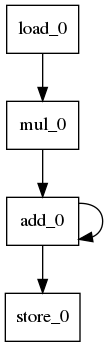
\includegraphics[scale=.2]{images/Architecture_latency_188_schematic.png}}
%\end{minipage}%
%\begin{minipage}{.5\linewidth}
%\centering
%\subfloat[]{\label{main:b}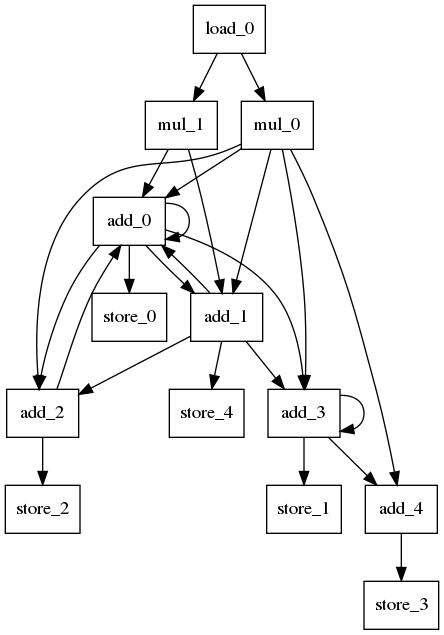
\includegraphics[scale=.2]{images/Architecture_latency_166_schematic.png}}
%\end{minipage}\par\medskip
%\centering
%\subfloat[]{\label{main:c}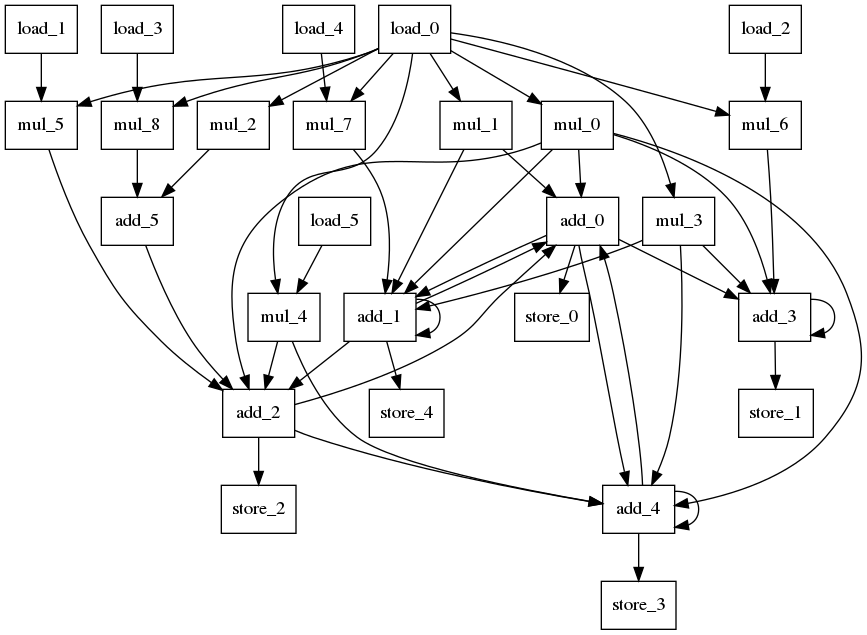
\includegraphics[scale=.10]{images/Architecture_latency_146_schematic.png}}
%
%\caption{my fig}
%\label{fig:main}
%\end{figure}

\vspace{-2mm}
\section{Architectural Template}
\label{sec:arch_template}
To implement the architectures generated by \frameworkname in hardware, we propose a PE template, shown in Figure~\ref{fig:FU_templ}. Each PE has an Instruction Memory (IM) where the operations to be performed at each clock cycle are stored. Each instruction is labeled with the clock cycle in which it should be scheduled. An internal clock counter is compared to the label to decide when to issue the instruction. The internal Register Files (RFs) are used to store input data that needs to be processed in the future, as well as output data that needs to be reused. The \textit{X-bar} in the diagram represent configurable crossbars, which can send data from any input port to any output port. OP is the hardware unit that performs an arithmetic (or logical) operation - e.g. add or multiply.
This PE template allows modular implementation of the spatial processor architecture - given that the instructions to execute are stored in the local IM. The inputs to a PE can either be generated by other PEs or the output generated by the same PE in the previous clock cycle. In addition, the inputs to the PE can be used as operands for immediate computation or stored in the RFs for future use. %We have implemented the template PE in RTL that can be configured to build all types of PEs found in the architectures generated by \frameworkname.

\begin{figure}[tb]
\centering
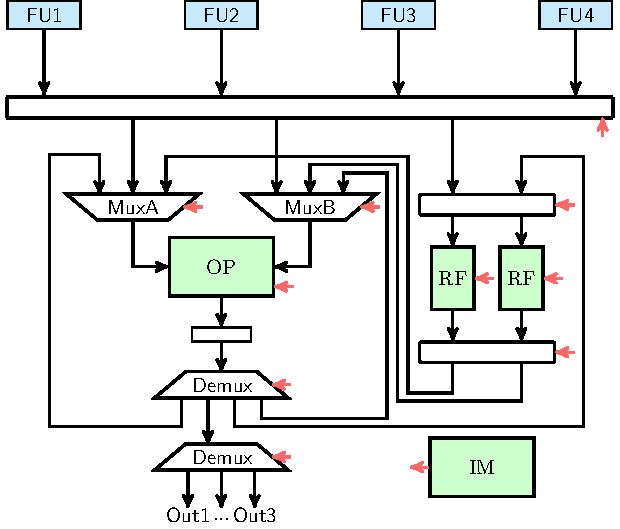
\includegraphics[width=.5\columnwidth]{images/functional_unit.pdf}
    \caption{\small Functional Unit template. PE1-PE4 represent "parent" PEs that generate input data. IM is an internal Instruction Memory,where the PE stores the operations to be performed. RFs are internal Register Files, which store reuse data and inputs to be used in the future. OP is the hardware unit actually performing the PE operation.}
\label{fig:FU_templ}
\squeezeup
\squeezeup
\end{figure}

\begin{figure*}[ht]
\centering
\begin{subfigure}{.33\textwidth}
  \centering
  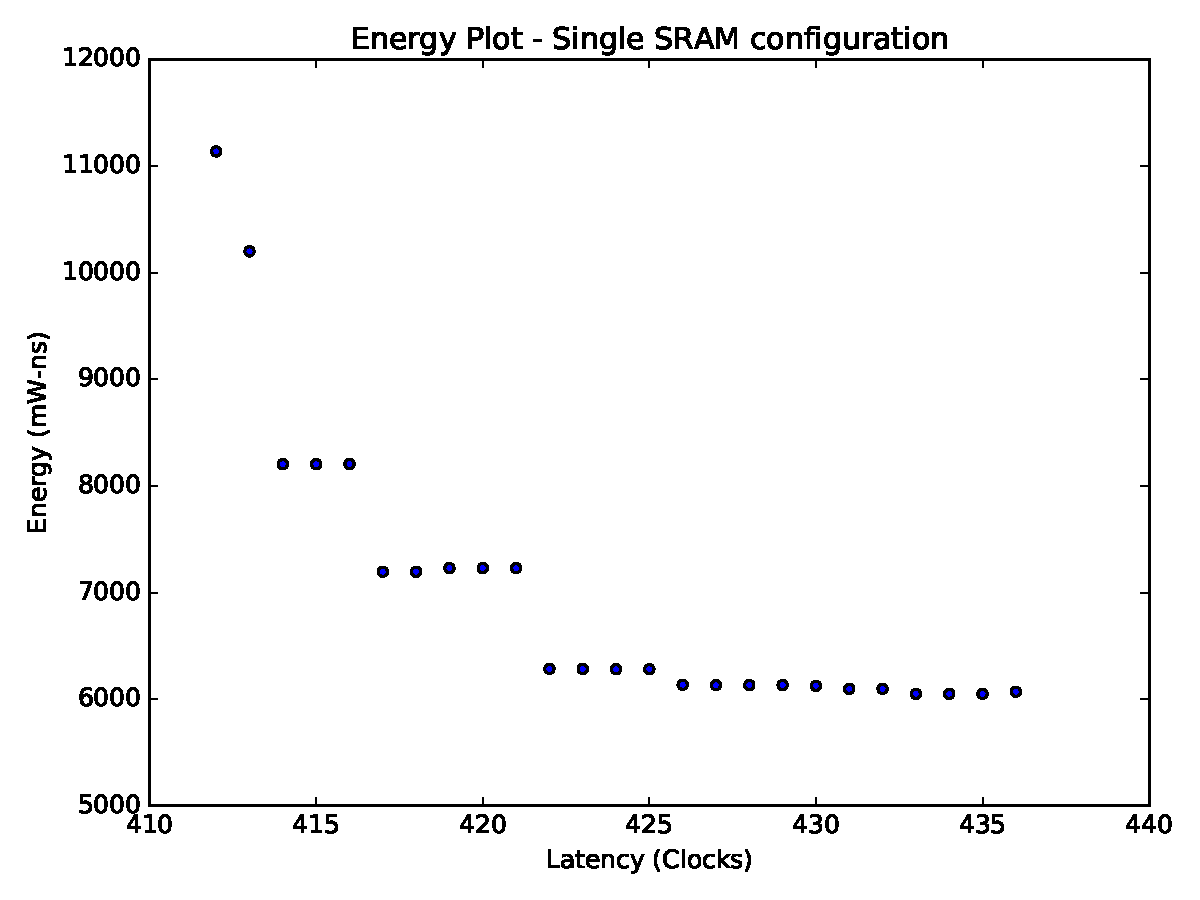
\includegraphics[width=\textwidth]{graphs/energy_plot_single_sram.pdf}
  \caption{5x5 MM}
  \label{fig:single_sram}
\end{subfigure}%
\begin{subfigure}{.33\textwidth}
  \centering
  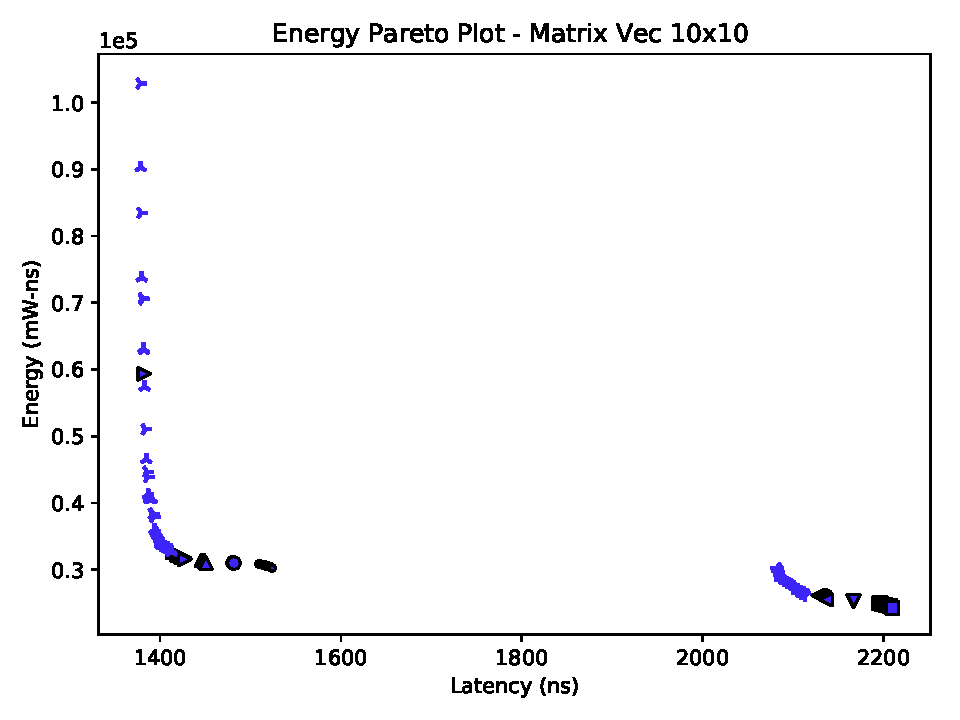
\includegraphics[width=\textwidth]{graphs/EnergyParetoMatrixVec10.pdf}
  \caption{MV 10x10}
  \label{fig:sram_vs_mram_pareto_vec}
\end{subfigure}
\begin{subfigure}{.33\textwidth}
  \centering
  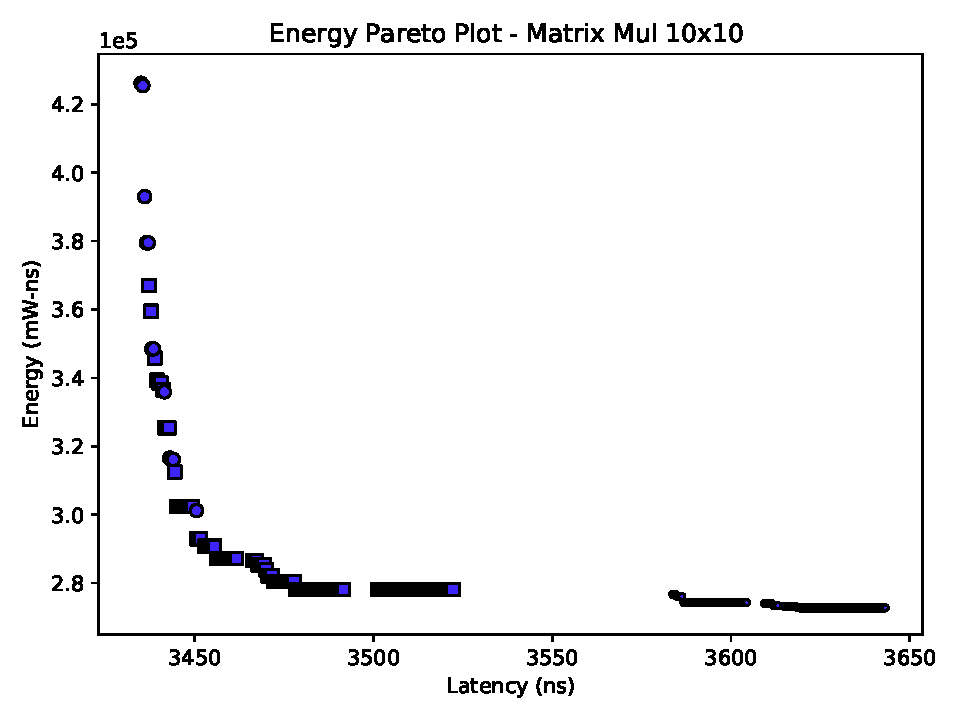
\includegraphics[width=\textwidth]{graphs/EnergyParetoMatrixMul10.pdf}
  \caption{MM 10x10}
  \label{fig:sram_vs_mram_pareto_mul}
\end{subfigure}
    \caption{\small Each point represents one \frameworkname~custom-processor. Different shapes (in \ref{fig:sram_vs_mram_pareto_vec} and~\ref{fig:sram_vs_mram_pareto_mul}) identify different input configurations. \ref{fig:single_sram} shows the architecture's Energy over Latency in clock cycles generated from a single configuration of a matrix vector multiplication of size 5x5. Note that (a) presents all designs, while (b) and (c) only include the Pareto-optimal designs.}
\label{fig:case_studies_1}
\end{figure*}
\section{Case Studies}
\label{sec:case_studies}
In this section we demonstrate the capabilities of \frameworkname~using three case studies. To do so, we analyze the architectures generated by \frameworkname~and we analyze the energy consumption and latency of each design.
We selected two representative applications: matrix-vector (MV) and matrix-matrix (MM) multiplication. The matrix sizes are 5x5, 10x10, and 15x15. We used the TSMC 28nm target technology library for generating the database containing the area usage and energy consumption of the different building blocks, as required by our framework.
We generated multiple input \textit{Configuration Parameters} - Section~\ref{ssec:conf_param} - to let \frameworkname~select the correct building blocks data from the database, and compute the latency, area usage, and energy consumption of the architectures. Each generated architecture has a known latency imposed in each iteration of the DSE(Section~\ref{ssec:dse}), which we use to compute its static energy consumption. Moreover, after applying the Modified Interval Partitioning algorithm (see Section~\ref{ssec:modified_interval_partitioning}), the instructions performed by each FU are known and this information is used to compute the dynamic energy consumption of an architecture. 

In the first case study - Section~\ref{ssec:exp_single} - we illustrate how DSE works for 5x5 MV and a single configuration. The second case study compares the use of MRAM - modeled according to~\cite{8310393} - and SRAM for L2M (both in 28nm) for the two applications. The last case study compares \frameworkname~architectures for the different MV sizes.

\vspace{-1mm}
\subsection{Single configuration DSE}
\label{ssec:exp_single}
\vspace{-1mm}
The goal of this case-study is to illustrate the ability of \frameworkname~to generate, given a single configuration, architectures with varying energy consumption. The configuration uses SRAM in both levels. L2M is clocked at 350MHz, while L1M and the custom processor are clocked at 1GHz. Figure 7a shows the energy consumption of 30 different \frameworkname~designs, with 30 latencies. We make two observations: (1) the designs' latencies and power consumption range between the min and max latency, as given by the \textbf{MostPar} and \textbf{MostSeq} architectures, and (2) as expected, faster designs exhibit higher energy consumption, due to their larger numbers of FUs.

%The \textbf{MostPar} - starting point of our DSE - is the fastest architecture completing the computation in 412 clock cycles of the custom processor and it consumes $11.1^3$ mW-ns. The \textbf{MostSeq} - ending point of the DSE - is the slowest, completing in 436 clock cycles and consuming $6^3$ mW-ns. Between these two extreme design points, the DSE generates intermediate architectures with various energy-latency tradeoffs. 

\vspace{-1mm}
\subsection{MRAM vs SRAM Level 2 Memory}
\label{ssec:case_study2}
\vspace{-1mm}

In this case study we compare the power efficiency of two alternative technologies to implement L2: MRAM and SRAM. 
The comparison is performed using both applications - MV and MM - with 10X10 matrices (see Fig~\ref{fig:sram_vs_mram_pareto_vec} and~\ref{fig:sram_vs_mram_pareto_vec}, respectively). In both graphs, each point is relative to a hardware architecture generated by \frameworkname; moreover shapes identify different input configurations. Specifically, we compare a total of 18 configurations: 2 L2M technologies, MRAM and SRAM, clocked at 350MHz, and 9 different clock frequencies (400MHz - 1GHz, in steps of 200) for the processor and L1M ensemble. 

In both figures we can identify two clusters: HE-LL (high-energy, low-latency) and LE-HL (low-energy, high-latency). Each cluster belongs to one memory technology: HE-LL contains of all SRAM designs, while LE-HL containts all MRAM designs. 
For the MV application (Fig~\ref{fig:sram_vs_mram_pareto_vec}) the fastest architecture - using SRAM memory - has a latency of 1375ns and consumes over $1^5$mW-ns. The most energy efficient SRAM architecture has instead a latency of 1525ns and consumes under $0.3^5$mW-ns, thus being 3x more energy efficient than the fastest with a 10\% increase in latency. The most energy efficient architecture using MRAM technology has instead a latency of 2210ns and consumes $0,24^5$mw-ns, hence having 45\% higher latency than the best SRAM counterpart, with 25\% decrease in power consumption. The matrix multiplication, Figure~\ref{fig:sram_vs_mram_pareto_mul}, performs 10 times more operation than the matrix vector multiplication, hence there is a clear overall increase in latency - about 30\% - and energy consumption - about 4 times -  in comparison to the previous application. In this case the architecture using SRAM consuming the least amount of energy is has 2\% higher latency compared to the fastest one, but consumes 50\% less energy. However, the introduction of MRAM technology in the L2M is not as beneficial as it was for the matrix vector application. The MRAM architecture consuming the least amount of energy has a 3\% slowdown compared to the most energy efficient SRAM, while attaining only a 2.2\% improvement in energy consumption. 

\subsection{Different Matrix Dimensions}
In this case study we compare three different matrix sizes for MV - 5x5, 10x10 and 15x15, using the same configurations used in~\ref{ssec:case_study2}, to evaluate how the energy consumption of an L2M MRAM scale with respect to an L2M SRAM. Figure~\ref{fig:sram_vs_mram_pareto_vec_sizes} shows the Pareto-optimal architectures generated from each input application. The increase in the matrix size is reflected by an increase in latencyi: all MV-5x5 custom-processors have latencies below 1000ns, MV-10x10 processors latencies range between 1250ns and 2500ns, and the MV-15x15 processors have latencies beyond 2500ns. 
However, the increased number of operations results instead in wider tradeoffs possibilities. Thus, the normalized latency gap between the most energy efficient SRAM and MRAM, decreases with the matrix size, from 82\% for the 5x5, to 42\% for the 10x10 and even 32\% for the 15x15. The reduction in energy consumption between the same pair of results is instead 20\% for the 5x5 and 10x10, while for the 15x15 drops to 16\%. Therefore, as the size of the matrix grows, the benefits in energy consumption when using MRAM technology in the L2M reduce. This is a behaviour caused by the increased number of write operations that have high energy impact when the MRAM technology is used. 

\begin{figure}[!h] 
\centering
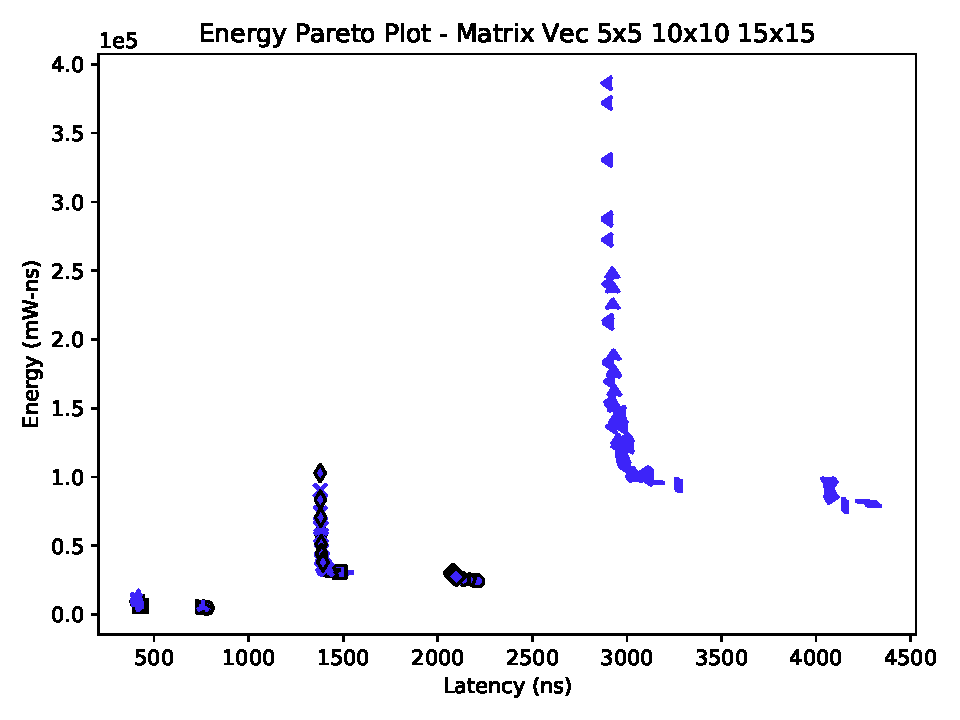
\includegraphics[width=0.33\textwidth]{graphs/EnergyParetoPlotMultipleSizeMAtrixVec.pdf}
    \caption{\small Energy Pareto optimal architectures generated by \frameworkname ~for different sizes of Matrix Vector multiplication 5x5 - with latencies ranging from 0 to 1000,10x10 - having latencies between 1000ns and 2500ns , and 15x15- with latencies above 2500ns. Each point corresponds to an architecture generated by the framework.}
\label{fig:sram_vs_mram_pareto_vec_sizes}
\end{figure}





\section{Related Work}

%Prior art on design-space exploration of custom or domain-specific processors~\cite{Jordans2014,EusseSAMOS2014,Jozwiak2013} aims to find the optimal processor architecture in terms of area usage, power consumption and execution cycles. Processors with Single Instruction Multiple Data (SIMD) or Single Instruction Multiple Threads (SIMT) are typically used for data-flow or streaming applications. SIMD and SIMT architectures are not scalable due to a single Instruction Memory. Spatial architectures~\cite{7284058,8686088} helps to distribute the Instruction Memory and achieve a higher clock speed. State-of-the-art Spatial archiectures are designed for maximum flexibility and provide connections from any ALU or PE to any other using an interconnect. Prior art on using non-volatile memories as a replacement L2 memory perform co-simulation of the processor and the memory system and optimizes the cache replacement policies~\cite{4798259,7092595,6271803,7360193,200116,Patel2016ReducingSL,Komalan:2014,Mittal13f}.

%For the energy model~\cite{Yannan2019}

%Papers to cite for CDFG generation and Application Specific High LSynthesis~\cite{Coussy:2008:HSA:1457713,Kato2008}



Previous work on designing spatial processor focuses on the hardware architecture of the processor, while the optimization of the memory system is only partially taken into account.
In \cite{parashar2014efficient} a spatial processor with distributed control across PE using triggered instructions is presented. Their architecture is built around the guarded-action programming paradigm, where guards - boolean expressions specifying if an action is legal - are evaluated by a scheduler and trigger computations. Support for high level languages is missing, so this spatial processor needs to be programmed in a low level guarded-action language and the computation needs to be manually mapped on the PEs. Their memory system consist of two levels of memories (L1 and L2) and distributed scratch-pad memories located within the PEs. The design is not tailored for a specific set of applications and they do not perform analysis on the interactions between the memory and processing systems, leaving the modeling of the memory system as future work.

Plasticine, a spatial processor optimized for the acceleration of parallel patterns is presented in \cite{prabhakar2017plasticine}. Their memory system is composed of Pattern Memory Units (PMUs) which are connected through a network to Pattern Compute Units (PCUs). Although it allows some degree of configuration, Plasticine is not meant to be optimized around specific applications. The input application needs to be written in a language exposing its parallel patterns - Delite Hardware Definition Language (DHDL) - and then it is mapped on the Plasticine architecture. Hence, the number of memory units (PMUs) and processing units (PCUs), and their interconnections are not optimized around specific applications.

In \cite{budiu2004spatial}, a framework to generate Application Specific Hardware (ASH) from a C application is presented. The final architecture it produces is asynchronous, and operation dependencies are handled using a token-based mechanism which is implemented in hardware. The memory system of the architecture consists of a monolithic memory. To handle concurrent memory requests the design uses a hierarchy of busses and arbiters, which creates a bottleneck. This means that their memory system is overwhelmed because it is not tailored for the PEs it uses.

Spatially distributed PEs with a dedicated configuration register allow to configure the PEs to one of the operating modes \cite{streamproc2019} at compile time. Few PEs are connected back-to-back, forming systolic arrays which are then interconnected using an on-chip interconnect. Thus, the processor architecture is quite general-purpose, i.e, the interconnect allows a PE array to be connected to any another PE array. However, there is no automated design flow to efficiently map algorithms to the processor architecture.

An interesting approach is Catena\cite{cerqueira2020catena}, an ultra-low-power spatial processor with a distributed architecture, where multiple techniques - \textit{clock gating}, \textit{power gating} and \textit{voltage boosting} - are applied in a fine-grained way to optimize energy efficiency. These techniques can be used to explore the power/latency tradeoff of specific applications. However, the impact of the memory system on the performance of the design is not modeled and the memory system is not co-designed with the spatial processor, potentially resulting in an inefficient utilization of the hardware resources; moreover, Catena lacks high-level language support.

In summary, a comparison of \frameworkname~against existing work is presented in Table \ref{tab:rw}.

\begin{table}[!ht]
 \resizebox{0.5\textwidth}{!}{%
\footnotesize
    \begin{tabular}{|l|l|l|l|l|l|}
      \hline
  Framework & Type    & Application & Memory & Architectural& High Level \\
           & (see \ref{sec:bg})    & Optimized & Co-Design &DSE & Language \\ \hline
\frameworkname         & Dist. Control       & Yes                   & Yes              & Yes               & Yes, C              \\ \hline
%            & Control       &                    &               &                &              \\ \hline
\cite{parashar2014efficient}               & Dist. Control       & No                    & No               & No                & No                  \\ \hline
%            & Control       &                    &                &                 &                   \\ \hline
\cite{prabhakar2017plasticine}               & Dist. Control       & No                    & No               & No                & Yes, DHDL         \\ \hline
            %&        &                     &                &                 & DHDL           \\ \hline
\cite{streamproc2019}               & Dist. Control       & No                    & No               & No                & No           \\ \hline
%            & Control       &                     &                &                 &            \\ \hline
\cite{budiu2004spatial}               & Logic & Yes                   & No               & No                & Yes, C \\
            & Grained &                    &                &                 &  \\ \hline
 \cite{cerqueira2020catena}              & Dist. Control  & Yes                   & No               & Yes                & No \\ \hline
%            & Control  &                    &                &                 &  \\ \hline
\end{tabular}
}
\caption{Comparison with related work.}
\label{tab:rw}
\end{table}

\section{Conclusion and Future Work}
In this work, we presented \frameworkname, a novel framework for co-designing memory-aware custom processors.
%with a two-level memory system. .
%Our framework enables the automatic design of a broad range of application-specific processors, using a two-level memory system.
The framework enables design-space exploration of spatial processor architectures including the memory system. We have empirically demonstrated that different spatial processor architectures can be quickly implemented using our novel PE hardware template. Lastly, we have shown the capabilities of the framework using three case studies, which illustrate the sanity of our DSE approach and its ability to facilitate a comparison between the use of MRAM and SRAM technologies.
For example, we were able to conclude that, for a matrix vector multiplication 10x10, the most energy efficient architecture generated with \frameworkname~with MRAM L2M has 45\% higher latency than the best SRAM counterpart, with 25\% decrease in power consumption.

Our future work focuses on the use \frameworkname~to analyze multiple applications. In addition, we plan to enhance our framework adding the capability of automatically \textit{merging} multiple spatial processor architectures, to generate a single \textit{multi-application spatial processor}.



\bibliographystyle{IEEEtran}
\bibliography{dsd20_biblio}


\vspace{12pt}


\end{document}
